%
% This is a borrowed LaTeX template file for lecture notes for CS267,
% Applications of Parallel Computing, UCBerkeley EECS Department.
%

\documentclass{article}
\usepackage{titlesec}
%\setlength{\oddsidemargin}{0.25 in}
%\setlength{\evensidemargin}{-0.25 in}
\setlength{\oddsidemargin}{0 in}
\setlength{\evensidemargin}{0 in}
\setlength{\topmargin}{-0.6 in}
\setlength{\textwidth}{6.5 in}
\setlength{\textheight}{8.5 in}
\setlength{\headsep}{0.75 in}
\setlength{\parindent}{0 in}
\setlength{\parskip}{0.1 in}


%
% ADD PACKAGES here:
%

\usepackage{amssymb}	% Already loads amsfonts
\usepackage{amsthm}
\usepackage{graphicx}
\usepackage{mathtools}	% Already loads amsmath
\usepackage{hyperref}
\usepackage{enumitem}
\usepackage{clrscode3e}  % for typesetting pseudocode
\usepackage{ulem}
\usepackage[usenames,dvipsnames]{xcolor}
\usepackage{multicol}


% Tikz and setup
\usepackage{tikz}
\usepackage{tikz-cd}
\usetikzlibrary{intersections, angles, quotes, calc, positioning}
\usetikzlibrary{arrows.meta}
\usepackage{pgfplots}
\pgfplotsset{compat=1.13}


\tikzset{
    force/.style={thick, {Circle[length=2pt]}-stealth, shorten <=-1pt}
}

%
% The following commands set up the lecnum (lecture number)
% counter and make various numbering schemes work relative
% to the lecture number.
%
\newcounter{lecnum}
\renewcommand{\thepage}{\thelecnum-\arabic{page}}
\renewcommand{\thesection}{\thelecnum.\arabic{section}}
\renewcommand{\theequation}{\thelecnum.\arabic{equation}}
\renewcommand{\thefigure}{\thelecnum.\arabic{figure}}
\renewcommand{\thetable}{\thelecnum.\arabic{table}}

%
% The following macro is used to generate the header.
%
\newcommand{\lecture}[5]{
   \pagestyle{myheadings}
   \thispagestyle{plain}
   \newpage
   \setcounter{lecnum}{#2}
   \setcounter{page}{1}
   \noindent
   \begin{center}
   \framebox{
      \vbox{\vspace{2mm}
    \hbox to 6.28in { {\bf #1
	\hfill} }
       \vspace{4mm}
       \hbox to 6.28in { {\Large \hfill Lecture #2: #3  \hfill} }
       \vspace{2mm}
       \hbox to 6.28in { {\it Lecturer: #4 \hfill Scribe: #5} }
      \vspace{2mm}}
   }
   \end{center}
   \markboth{Lecture #2: #3}{Lecture #2: #3}
   \vspace*{4mm}
}
\renewcommand{\cite}[1]{[#1]}
\def\beginrefs{\begin{list}%
        {[\arabic{equation}]}{\usecounter{equation}
         \setlength{\leftmargin}{2.0truecm}\setlength{\labelsep}{0.4truecm}%
         \setlength{\labelwidth}{1.6truecm}}}
\def\endrefs{\end{list}}
\def\bibentry#1{\item[\hbox{[#1]}]}

\newcommand{\fig}[3]{
			\vspace{#2}
			\begin{center}
			Figure \thelecnum.#1:~#3
			\end{center}
	}

% Colored theorem styles
\makeatother
\usepackage{thmtools}
\usepackage[framemethod=TikZ]{mdframed}
\mdfsetup{skipabove=1em,skipbelow=1em}

\declaretheoremstyle[
    headfont=\bfseries\sffamily\color{ForestGreen!70!black}, bodyfont=\normalfont,
    mdframed={
        linewidth=2pt,
        rightline=false, topline=false, bottomline=false,
        linecolor=ForestGreen, backgroundcolor=ForestGreen!5,
    },
    spaceabove=8pt
]{thmgreenbox}

\declaretheoremstyle[
    headfont=\bfseries\sffamily\color{NavyBlue!70!black}, bodyfont=\normalfont,
    mdframed={
        linewidth=2pt,
        rightline=false, topline=false, bottomline=false,
        linecolor=NavyBlue, backgroundcolor=NavyBlue!5,
    },
    spaceabove=8pt
]{thmbluebox}

\declaretheoremstyle[
    headfont=\bfseries\sffamily\color{NavyBlue!70!black}, bodyfont=\normalfont,
    mdframed={
        linewidth=2pt,
        rightline=false, topline=false, bottomline=false,
        linecolor=NavyBlue
    },
    spaceabove=8pt
]{thmblueline}

\declaretheoremstyle[
    headfont=\bfseries\sffamily\color{RawSienna!70!black}, bodyfont=\normalfont,
    mdframed={
        linewidth=2pt,
        rightline=false, topline=false, bottomline=false,
        linecolor=RawSienna, backgroundcolor=RawSienna!5,
    },
    spaceabove=8pt
]{thmredbox}

\declaretheoremstyle[
    headfont=\bfseries\sffamily\color{RawSienna!70!black}, bodyfont=\normalfont,
    numbered=no,
    mdframed={
        linewidth=2pt,
        rightline=false, topline=false, bottomline=false,
        linecolor=RawSienna, backgroundcolor=RawSienna!1,
    },
    qed=\qedsymbol,
    spaceabove=8pt
]{thmproofbox}

\declaretheoremstyle[
    headfont=\bfseries\sffamily\color{NavyBlue!70!black}, bodyfont=\normalfont,
    numbered=no,
    mdframed={
        linewidth=2pt,
        rightline=false, topline=false, bottomline=false,
        linecolor=NavyBlue, backgroundcolor=NavyBlue!1,
    },
    spaceabove=8pt
]{thmexplanationbox}

% Use these for theorems, lemmas, proofs, etc.
\theoremstyle{definition}
\declaretheorem[style=thmgreenbox, name=Definition, numberwithin=lecnum]{definition}
\declaretheorem[style=thmbluebox, numbered=no, name=Example]{example}
\declaretheorem[style=thmredbox, name=Theorem, numberwithin=lecnum]{theorem}
\declaretheorem[style=thmredbox, name=Proposition, sibling=theorem]{proposition}
\declaretheorem[style=thmredbox, name=Lemma, sibling=theorem]{lemma}
\declaretheorem[style=thmredbox, name=Corollary, sibling=theorem]{corollary}
% \newtheorem{theorem}{Theorem}[lecnum]
% \newtheorem{lemma}[theorem]{Lemma}
% \newtheorem{claim}[theorem]{Claim}
% \newtheorem{corollary}[theorem]{Corollary}
% \newtheorem{definition}[theorem]{Definition}
\declaretheorem[style=thmblueline, numbered=no, name=Remark]{remark}
\renewenvironment{proof}{{\bf \textit{Proof.}}}{\hfill\rule{2mm}{2mm}}
\makeatletter


% **** IF YOU WANT TO DEFINE ADDITIONAL MACROS FOR YOURSELF, PUT THEM HERE:

\renewcommand\Pr{\mathbb{P}}
\newcommand\Ex{\mathbb{E}}

\newcommand\N{\mathbb{N}}
\newcommand\Z{\mathbb{Z}}
\newcommand\Q{\mathbb{Q}}
\newcommand\R{\mathbb{R}}
\newcommand\C{\mathbb{C}}
\newcommand\F{\mathbb{F}}

\DeclarePairedDelimiter\ceil{\lceil}{\rceil}
\DeclarePairedDelimiter\floor{\lfloor}{\rfloor}
\DeclarePairedDelimiter\anglebrac{\langle}{\rangle}

\begin{document}
\lecture{MAT344 Intro to Combinatorics}{1}{Strings, Enumeration, and Permuation}{Reila Zheng}{Kevin Gao}

\textbf{Q}: How many outcomes ar ethere if you roll a die and toss a coin? \\
\textbf{A}: \# of outcomes for a die: 6; \# of outcomes for a coin: 2; Hence, $6 \times 2 = 12$

\textbf{Q}: How many outcomes are there if you either roll a die or toss a coin? \\
\textbf{A}: $6 + 2 = 8$ 

\textbf{Q}: How many ways to get from home to Bahen without backtracking?
\begin{figure}[htbp]
   \centering
   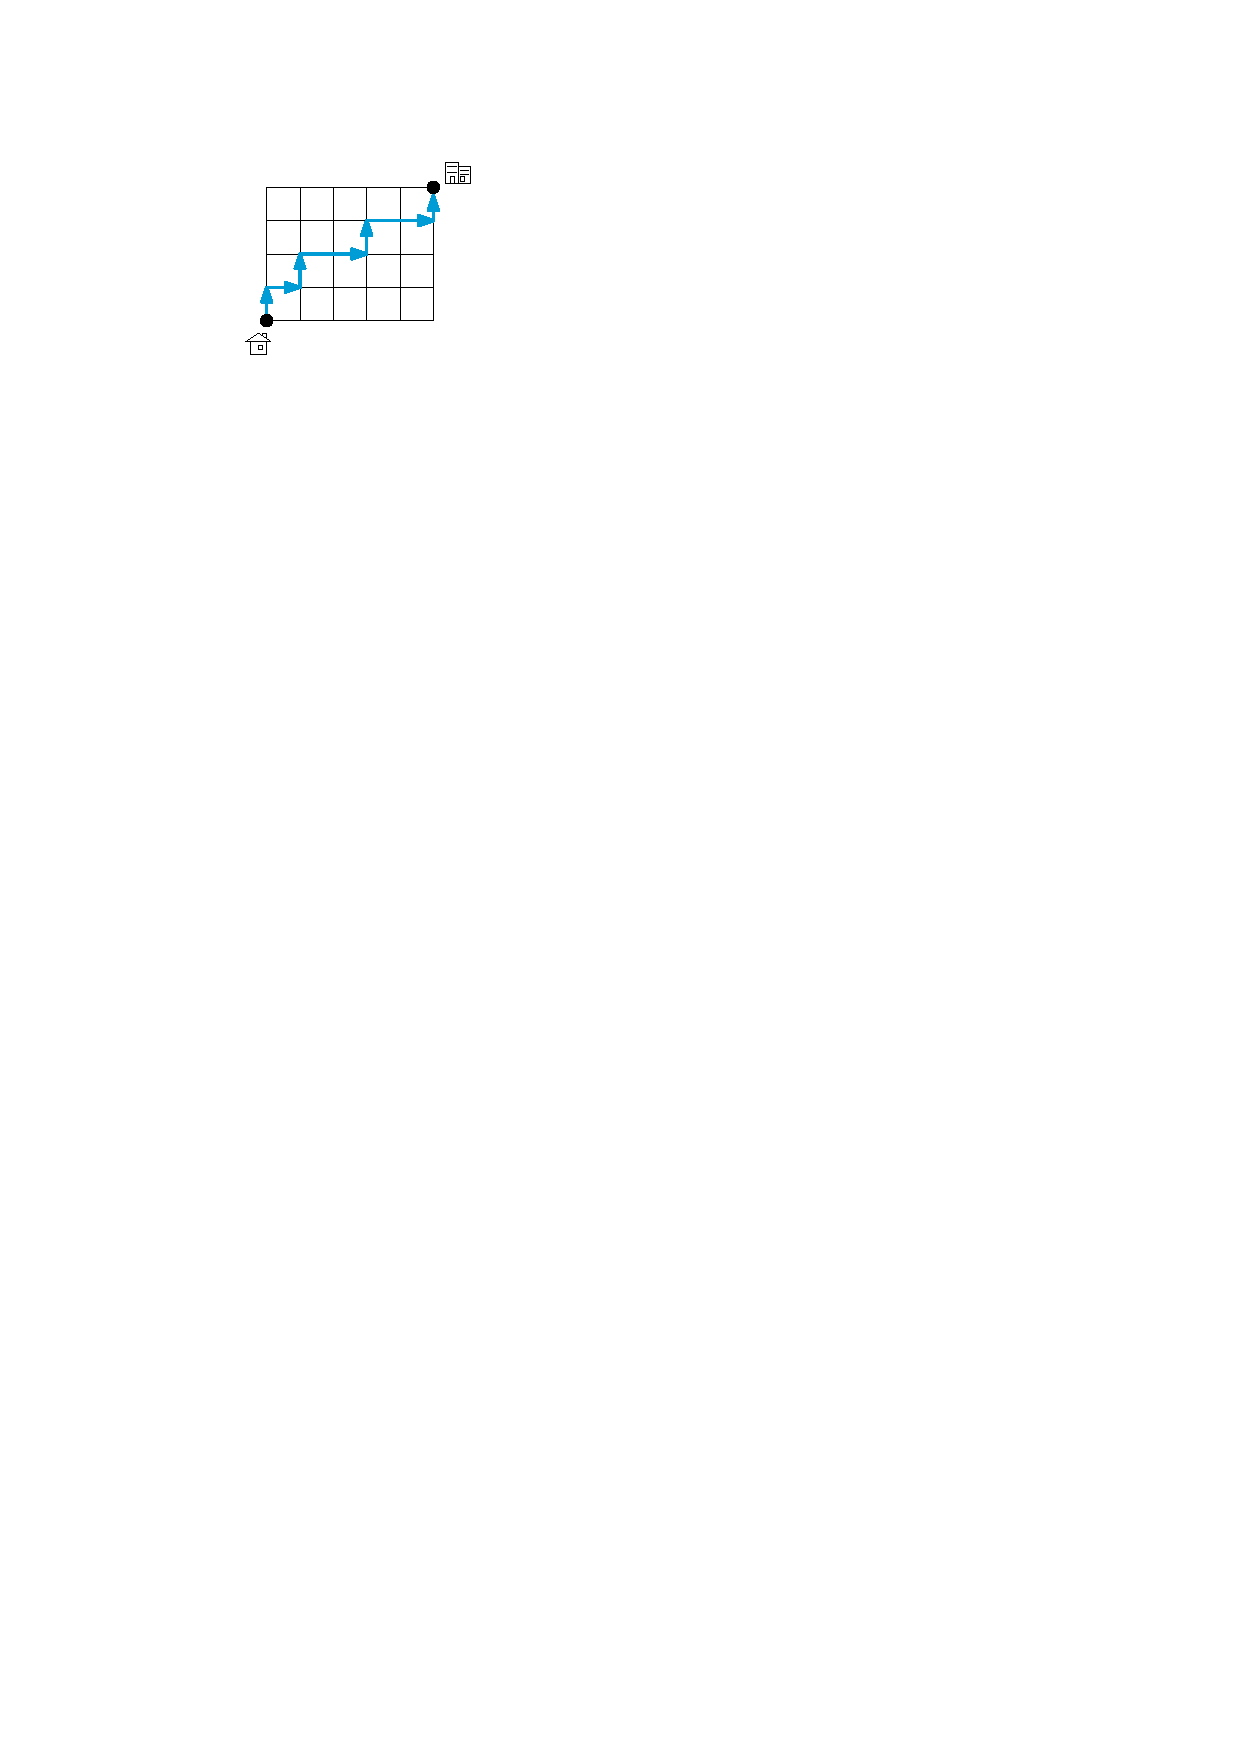
\includegraphics[width=0.3\linewidth]{figures/house-to-bahen-path.pdf}
   \label{fig:home-to-bahen}
\end{figure}

\section{Strings}

\begin{definition}[Binary String]
   A \textit{\textbf{binary string}} of length $n$ is an ordered list of length $n$ of elements from $\{0,1\}$. 
\end{definition}

\begin{example}
   $10011$ is a binary string of length $5$. $\emptyset = \{\}$ is a binary string of length $0$.
\end{example}

Similarly, a \textit{\textbf{ternary string}} of length $n$ is an ordered list of length $n$ of elements from $\{0,1,2\}$.

\begin{definition}[X-String]
   Let $X = \{a_1,\ldots,a_n\}$ be the alphabet. An $X$-string of length $k$ is an ordered list of elements from the set $X$.
\end{definition}

In the previous example, the path from home to Bahen without backtracking can be thought of as an $\{\text{N},\text{E}\}$-strings.

\textbf{Q}: How to relate the set of paths from home to Bahen without backtracking with some set of $\{\text{N},\text{E}\}$-strings? \\
\textbf{A}: Note that not every $\{\text{N},\text{E}\}$-strings can represent a path. In our specific examples, we need exactly walk $5$ blocks east and $4$ blocks north.

\textbf{Q}: How many $\{\text{N},\text{E}\}$-strings of length $9$ are there? \\
\textbf{A}: Let $\mathcal{S} = \{\text{all $\{$N, E$\}$-strings of length 9}\}$. For each $S \in \mathcal{S}$, $S = s_1s_2\ldots s_9$. For each position, there are two choices, N or E. Hence, there are $2^9$ possible $\{\text{N},\text{E}\}$-strings in $\mathcal{S}$.

\begin{theorem}
   For $X = \{a_1,\ldots,a_n\}$, the number of $X$-strings of length $k$ is $n^k$, where $n,k \geq 1$ are natural numbers.
\end{theorem}

\begin{proof}
   Denote $S = s_1\ldots s_k \in \mathcal{S}$. For $s_i$, there are $n$ choices for $i \in \{1, \ldots, k\}$. So there are
   $$
   \underbrace{n \times n \times \cdots \times n}_{\text{$k$ times}} = n^k
   $$
   such strings.
\end{proof}

\begin{definition}[Array]
   An \textit{\textbf{array}} of length $n$ is an ordered list where the elements in position $i$ comes from some alphabet $X_i$.
\end{definition}

\begin{example}
   Ontario health cards have the format: 10 digits of $\{0,1,\ldots,9\}$ followed by two letters from $\mathrm{\{A,\ldots,Z\}}$. There are $(10)^{10} \times (26)^2$ possible health card numbers.
\end{example}

\section{Permutations}

Let $X = \{a_1,\ldots,a_n \}$ be a set of distinct object.

\begin{definition}[Permutation]
   A \textit{\textbf{permutation}} of length $k$ is an $X$-string of length $k$ such that there is no repetition. Equivalently, $s$ is injectively.

   Given integers $n$ and $k$ with $n \geq k$, we let $P(n,k)$ denote the number of permuations of $[n]$ of length $k$.
\end{definition}

\begin{example}
   Suppose $X = \{a,b,c,d\}$. $abc$ is a permutation of length 3. $\emptyset$ is a permutation of length 0. However, $bab$ is not a permutation because of the repeating character $b$.
\end{example}

\begin{remark}
   Because a permutation requires there be no repetition, there is no permutation of length $k$ for $X$ of size $n$ if $k > n$.
\end{remark}

\textbf{Q}: How many permutations of length 4 are there of $X = \{a,b,c,d\}$? \\
\textbf{A}: Let $S = s_1s_2s_3s_4$ be a permutation. There are 4 choices for $s_1$. After choosing $s_1$, there are 3 choices left for $s_2$. After choosing $s_2$, there are 2 choices left for $s_3$. Similarly, after choosing $s_3$, there is 1 choice left for $s_4$. In total, there are $4 \times 3 \times 2 \times 1$ permutations for $\{a,b,c,d\}$.

\begin{definition}[Factorial]
   For any $n \in \N$ such that $n \geq 0$, $n$ \textit{\textbf{factorial}} is defined as
   $$
   n! = n \times (n-1) \times (n-2) \times \cdots \times 2 \times 1
   $$
   In particular, we define $0! = 1$.
\end{definition}

We use $P(n,k)$ to denote the number of permutations of $[n]$ of length $k$ (i.e. $[n] = \{0,1,\ldots,n\}$).

For example, consider the number of permutations of $[3]$.

\textbf{Q}: What are the permutations of length 2 for $[3]$? \\
\textbf{A}: 01, 02, 12, 10, 20, 21

\textbf{Q}: What are the number of permutations of length 3 of $[3]$? \\
\textbf{A}: 012, 021, 102, 120, 210, 201

\textit{Observation}: There are the same number of permutations of $[3]$ of length 3 as the number of permutations of $[3]$ of length 2.

Then, it is natural to ask if we can generalize this. That is, when is $P(n,k)=P(n,k')$?

Consider a permutation of $[3]$ of length 3, $p = p_1p_2$. For $p_1$, there are 3 choices. After choosing $p_1$, there are 2 choices for $p_2$. So, in total, there are $3 \times 2$ permutations of $[3]$ of length 2.

Now, consider a permutation of $[3]$ of length 3, $p = p_1p_2p_3$. For $p_1$, there are 3 choices. After choosing $p_1$, there are 2 choices for $p_2$. After choosing $p_1$ and $p_2$, there is exactly 1 choice for $p_3$. In total, there are $3 \times 2 \times 1$ choices for $p$, a permutation of length $3$ of $[3]$.

\begin{proposition}
   For $n \geq 1$,
   $$
   P(n,n) = P(n,n-1)
   $$
\end{proposition}
\begin{proof}
   The proof is similar to how we showed $P(3,3)=P(3,2)$.
\end{proof}

Next, we ask if there are any other $k=k'$ for some $k,k' \leq n$ and $n\geq 1$ such that $P(n,k) = P(n,k')$.

One common technique in combinatorics is to find a bijective correspondance from one set to another. To show that $P(3,2)=P(3,3)$, we can find a bijective correspondance as shown in the figure below

\begin{figure}[h]
   \centering
   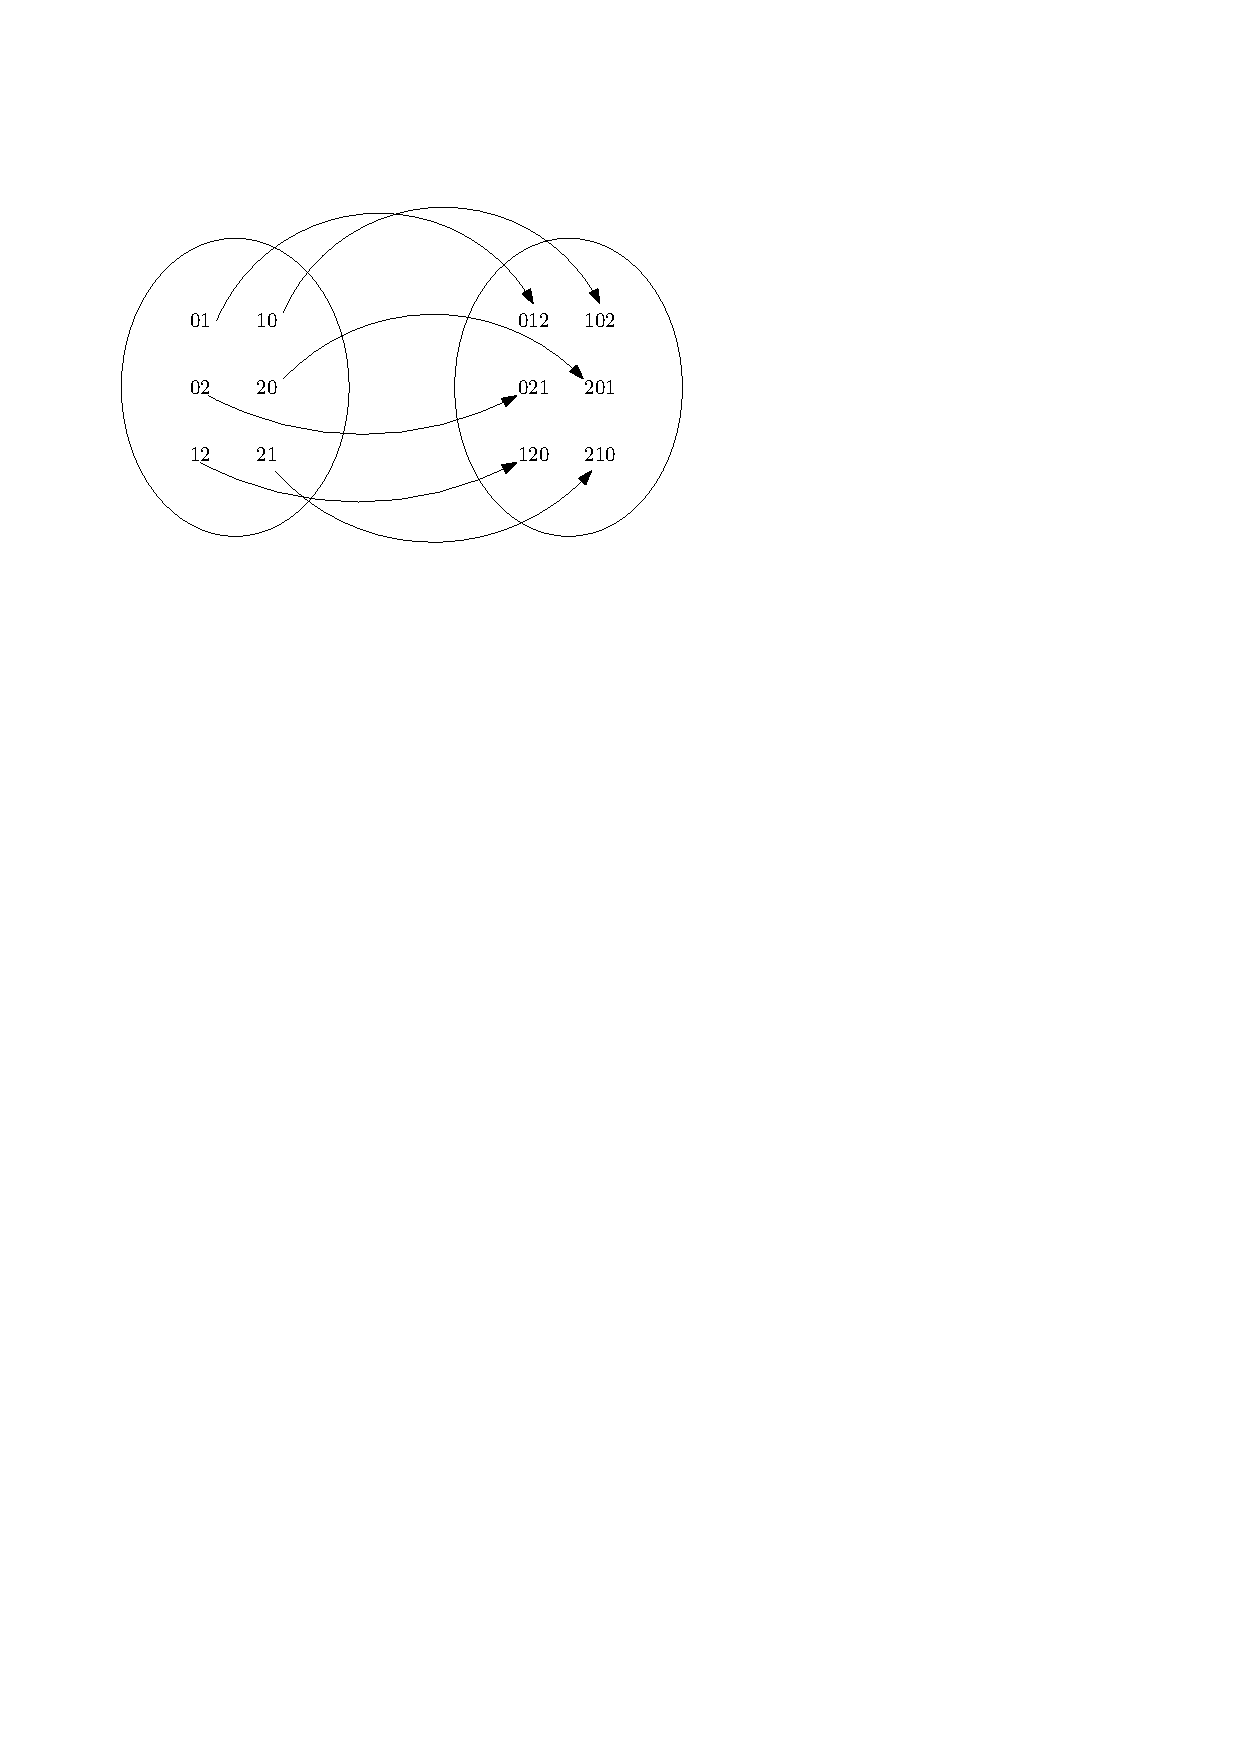
\includegraphics[width=0.4\linewidth]{figures/biject-correspondance.pdf}
   \caption{Bijective correspondance showing $P(3,2)=P(3,3)$.}
\end{figure}

\begin{theorem}
   Given integers $n$ and $k$ with $n \geq k$,
   $$
   P(n,k) = \frac{n!}{(n-k)!}
   $$
\end{theorem}

\begin{proof}
   Consider $p=p_1p_2\cdots p_k$, a permutation of $[n]$ of length $k$. For $p_1$, there are $n$ choices. After choosing $p_1$, there are $n-1$ choices for $p_2$. In general, after choosing $p_i$, there are $n-i$ choices for $p_{i+1}$. We repeat this until we get $p_k$. In total, we have
   $$
   P(n,k) = n \times \cdots \times (n-(k-1)) = \frac{n!}{(n-k)!}
   $$

   Alternatively, we can prove this by fixing $n$ and induct on $k$.
\end{proof}

From this theorem, we get the same result that $P(n,n) = P(n,n-1)$.
\begin{corollary}
   $$
   P(n,n-1) = P(n,n)
   $$
\end{corollary}
\begin{proof}
   $$
   P(n,n) = \frac{n!}{(n-n)!} = n!
   $$
   $$
   P(n,n-1) = \frac{n!}{(n-(n-1))!} = \frac{n!}{1!} = n!
   $$
\end{proof}

\lecture{MAT344 Intro to Combinatorics}{2}{Combinations}{Reila Zheng}{Kevin Gao}

\section{Subsets and Combination}

\begin{definition}[Combination]
   Given a set of objects $X$, a combination of size $k$ is a subset $A \subseteq X$ of size $k$.
\end{definition}

\begin{example}
   What are the subsets of $\{1,2,3\}$?
   $$
   \emptyset=\{\}, \{1\}, \{2\}, \{3\}, \{1,2\}, \{1,3\}, \{2,3\}, \{1,2,3\}
   $$
   There are 3 combinations of $\{1,2,3\}$ of size 2.
\end{example}

Set notations:
\begin{multicols}{3}
   $\emptyset$ or $\varnothing$: empty set; \\
   $\in$: element of; \\
   $\subset$: subset of; \\
   $\subseteq$: subset of; \\
   $\subseteq$: proper subset of; \\
   $\not\in$: not an element of
\end{multicols}

\begin{remark}
   For elements of a set, order does not matter.
\end{remark}

Another example
\begin{example}
   Say we have $X=\{a,b,c,d\}$. $\emptyset$ is the unique combination of $X$ of size $0$. $\{a,d\}$ and $\{b,a\}$ are the combinations of $X$ of size 2.
\end{example}

In general, we use the following notation
\begin{definition}
   $C(n,k)$ is the number of combinations of $[n]$ of size $k$ where $0 \leq k \leq k$ are integers.
\end{definition}

\begin{remark}
   Note that as with the case for permutation, there are no combinations of $[n]$ of size $k > n$.
\end{remark}

\textbf{Q}: What is the value of $C(n,k)$? \\
\textbf{A}: Intuitively, there should be more permutations than combinations because order matters for permutations.

Consider the combinations of $[4]$ of size $2$. They are $\{0,1\}, \{0,2\}, \{0,3\}, \{1,2\}, \{1,3\}, \{2,3\}$. So there are 6 combinations. Note that for each combination, we can order it in $2!$ ways, giving us $6 \cdot 2!$ permutations.

\begin{theorem}
   For $n \geq k \geq 0$,
   $$
   C(n,k) = \frac{P(n,k)}{k!}
   $$
\end{theorem}

\begin{proof}
   We will show that for any combination $A$ of $[n]$ of size $k$, there are $k!$ ways to order the elements into permutations of size $k$.

   Note that given a permutation $p = p_1\cdots p_k$, there is exactly one such set $A = \{p_1,\ldots,p_k\}$ because the elements in a permutation do not repeat. Of the $k!$ permutations of $A$, each one is a permutation of $[n]$ of length $k$.

   Hence, there are $C(n,k)$ combinations, and there are $k!$ ways to order each combination such that we get a unique permutation. All such permutations can be obtained this way.

   Therefore, $P(n,k) = C(n,k) \cdot k!$ (the number of permutations is the number of combinations times the number of ways to order each combination), and the theorem follows.
\end{proof}

An alternative notation for $n$ choose $k$ is
$$
C(n,k) = \binom{n}{k} = \frac{n!}{(n-1)!k!}
$$

\begin{corollary}
   $C(n,k) = C(n,n-k)$.
\end{corollary}

\begin{proof}
   Trivially follows from the formula.
\end{proof}

Combinatorially, if we choose $k$ elements of $[n]$ (i.e. tagging them with 1), then the number of ways to tag the ones we chose is the same as the number of ways to tag the ones we did not choose.

\begin{remark}
   $\binom{n}{k}$ are the binomial coefficients. This means the coefficient of $x^k$ in the expansion of $(1+x)^n$ is exactly $\binom{n}{k}$. 
\end{remark}
Intuitively,
$$
\underbrace{(1+x) \cdots \cdots (1+x)}_{\text{$n$ terms}}
$$
for the $x^k$ term, we take $x$ exactly $k$ times and take 1 exactly $n-k$ times.

\section{Applications}

Let us revisit one of the motivating examples at the beginning.

\textbf{Q}: How many ways to get from home to Bahen without backtracking? \\
\textbf{A}: There are 9 steps we need to take. 5 of those 9 steps need to be going to the east, and 4 of the 9 steps need to be going to the north. More formally, we need the number of $\{\text{N,E}\}$-strings of length 9 with 4 N's. This is equivalent to choosing 4 positions/indicies to place the N's or 5 positions/indicies to place the E's. So, in total, we have $\binom{9}{4} = \binom{9}{5}$ paths.

\section{Bijective Correspondance}

Suppose we have sets $A$ and $B$. $f:\;A\to B$ is a function.

\begin{definition}[Injective]
   We say $f$ is injective or one-to-one if $\forall a_1\neq a_2 \in A.\, f(a_1) \neq f(a_2)$.
\end{definition}

\begin{definition}[Surjective]
   We say $f$ is surjective or onto if $\forall b \in B.\, \exists a \in A.\, f(a) = b$.
\end{definition}

\begin{definition}[Bijection]
   We say that $f$ is bijective if $f$ is both injective and surjective.
\end{definition}

\begin{remark}
   If there is a bijective mapping $f:\; A \to B$, then $A$ and $B$ have the same size (cardinality).
\end{remark}

This is useful because it allows us to count things using things that we already know how to count if we can find a bijection between the two sets.

\end{document}